\documentclass[tikz,border=2pt]{standalone}
\usepackage{times}
\usepackage{amsmath,amssymb}
\usetikzlibrary{positioning,arrows.meta}
\begin{document}
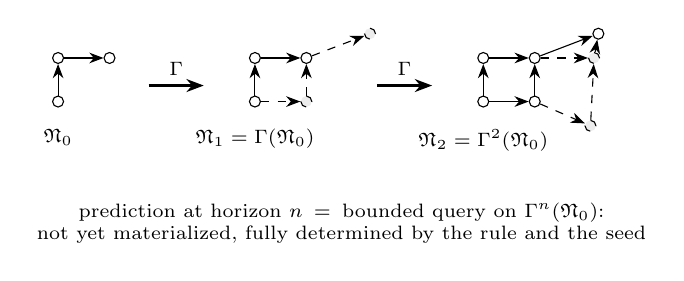
\begin{tikzpicture}[font=\scriptsize,
  v/.style={circle, draw, inner sep=1.4pt, fill=white},
  nv/.style={circle, draw, dashed, inner sep=1.4pt, fill=gray!15},
  e/.style={-{Stealth[length=1.8mm]}},
  ne/.style={-{Stealth[length=1.8mm]}, dashed}]
\begin{scope}
\node[v] (a0) {}; \node[v, right=5mm of a0] (b0) {};
\node[v, below=4mm of a0] (c0) {};
\draw[e] (a0)--(b0); \draw[e] (c0)--(a0);
\node[below=1.5mm of c0] {$\mathfrak{N}_0$};
\end{scope}
\draw[-{Stealth[length=2.2mm]}, thick] (1.15,-0.35) -- node[above]{$\Gamma$} (1.85,-0.35);
\begin{scope}[xshift=25mm]
\node[v] (a1) {}; \node[v, right=5mm of a1] (b1) {};
\node[v, below=4mm of a1] (c1) {};
\node[nv, right=5mm of c1] (d1) {}; \node[nv, above right=2mm and 7mm of b1] (e1) {};
\draw[e] (a1)--(b1); \draw[e] (c1)--(a1);
\draw[ne] (c1)--(d1); \draw[ne] (d1)--(b1); \draw[ne] (b1)--(e1);
\node[below=1.5mm of c1] {$\mathfrak{N}_1=\Gamma(\mathfrak{N}_0)$};
\end{scope}
\draw[-{Stealth[length=2.2mm]}, thick] (4.05,-0.35) -- node[above]{$\Gamma$} (4.75,-0.35);
\begin{scope}[xshift=54mm]
\node[v] (a2) {}; \node[v, right=5mm of a2] (b2) {};
\node[v, below=4mm of a2] (c2) {};
\node[v, right=5mm of c2] (d2) {}; \node[v, above right=2mm and 7mm of b2] (e2) {};
\node[nv, below right=2mm and 6mm of d2] (f2) {}; \node[nv, right=6mm of b2] (g2) {};
\draw[e] (a2)--(b2); \draw[e] (c2)--(a2); \draw[e] (c2)--(d2); \draw[e] (d2)--(b2); \draw[e] (b2)--(e2);
\draw[ne] (d2)--(f2); \draw[ne] (g2)--(e2); \draw[ne] (b2)--(g2); \draw[ne] (f2)--(g2);
\node[below=1.5mm of c2] {$\mathfrak{N}_2=\Gamma^{2}(\mathfrak{N}_0)$};
\end{scope}
\node[align=center, font=\scriptsize] at (3.6,-2.1) {prediction at horizon $n$ \,=\, bounded query on $\Gamma^{n}(\mathfrak{N}_0)$:\\ not yet materialized, fully determined by the rule and the seed};
\end{tikzpicture}
\end{document}
